\documentclass[9pt, letterpaper]{article}
\usepackage[utf8]{inputenc}
\usepackage{graphicx} %package to manage images
\usepackage{wrapfig}
\usepackage{multicol}
\setlength{\columnsep}{1cm}
\usepackage[margin=0.18in]{geometry}
\title{301 Cheat Sheet}
\author{Tramwreck Nguyen, Renae Sassmaster Taylor, and Ariel Oelsnerd}
\date{September 2017}
\begin{document}
\textbf{temporal locality} if a data location is referenced then it will tend to be referenced again soon. \textbf{spatial locality} if a data location is referenced, data locations with nearby addresses will tend to be referenced soon. \textbf{memory hierarchy} a structure that uses multiple levels of memories; as the distance from the processor increases, the size of the memories and the access time both increase.  \textbf{block} minimum unit of information that can be either present or not present in a cache. 
\textbf{hit time} the time required to access a level of the memory hierarchy, including the time needed to determine whether the access is a hit or a miss. \textbf{miss penalty} the time required to fetch a block into a level of the memory hierarchy from the lower level, including time to access the block, transmit it from one level to the other, insert it in the level that experienced the miss, and then pass the block to the requestor.\\
A \textbf{direct-mapped cache} structure in which each memory location is mapped to exactly one location in the cache.\\ \textbf{tag} A field in a table used for a memory hierarchy that contains the address information required
to identify whether the associated block in the hierarchy corresponds to a requested word. Bigger blocks $\to$ lower miss rate but higher miss penalty. \\
Note for self: it's a hit if same tag, same index. A replacement if same index, same offset (if exists), different tag. 4Kib = $2^{10}$ words.\\
%\begin{multicols}{3}
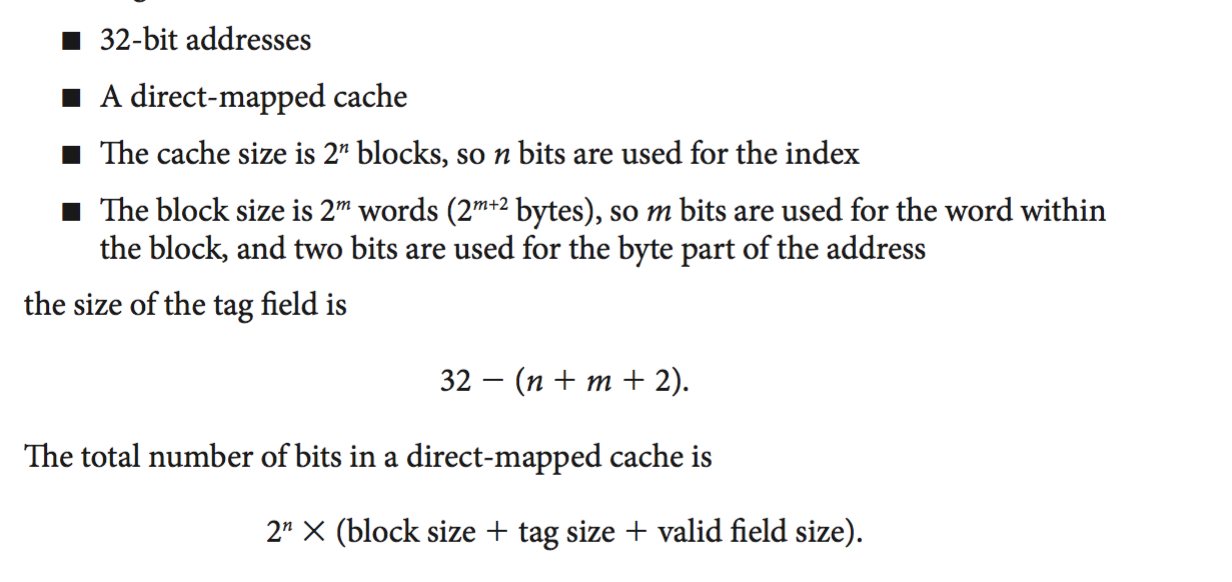
\includegraphics[scale=0.35]{blockSizeFormula.png}
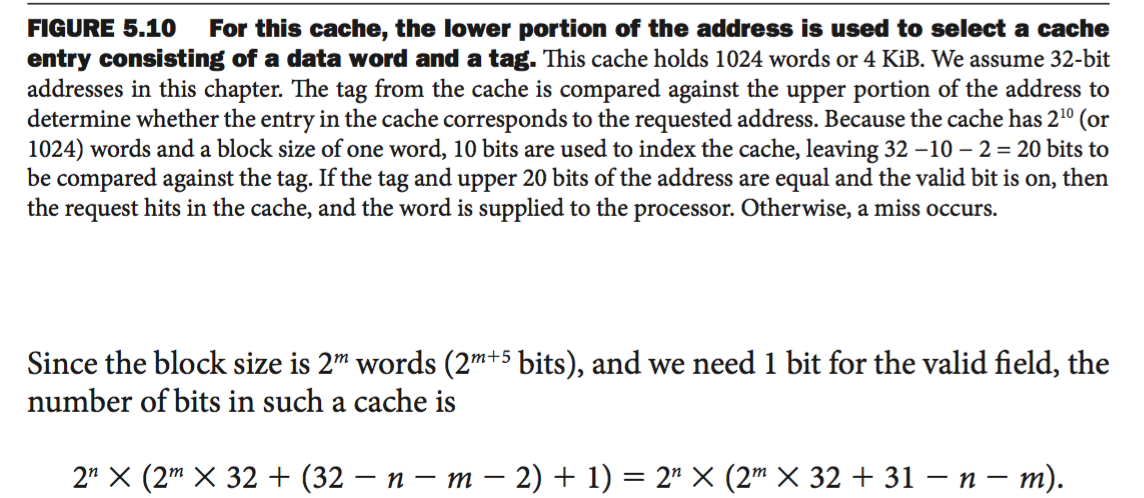
\includegraphics[scale=0.4]{blockSize.png}
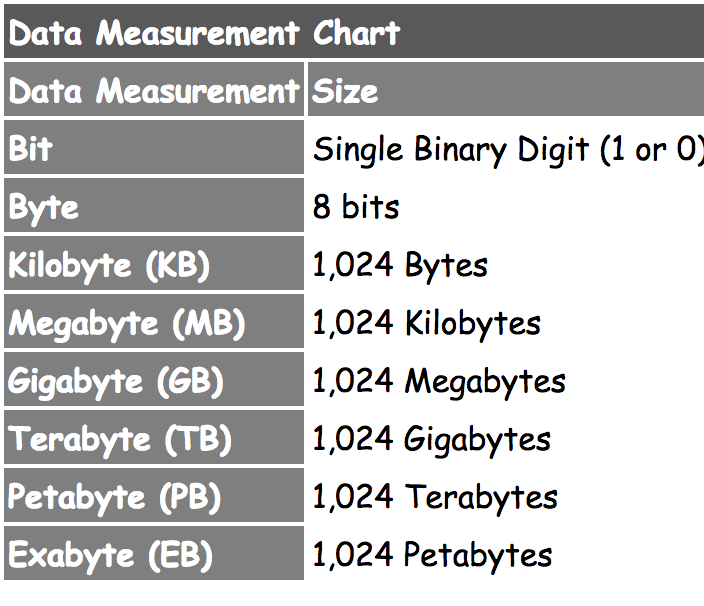
\includegraphics[scale=0.35]{Bytes}\\
%\end{multicols}
\textbf{write-through} writes always update both the cache and the next lower level of the memory hierarchy, ensuring that data is always consistent between the two. \textbf{write buffer} A queue that holds data while the data is waiting to be written to memory. \textbf{write-back} The new value is written only to the block in the cache,  the modified block is written to the lower level of the hierarchy when it is replaced.\\
CPU time = (CPU execution clock cycles [including cache hits] + Memory-stall clock cycles [cache misses]) x Clock cycle time.\\
Memory-stall clock cycles =  (Read-stall cycles  + Write-stall cycles), Read-stall cycles = $\frac{Reads}{Program}$ x Read miss rate x  Read miss penalty.\\
Write-stall cycles = $\frac{Writes}{Program}$x Write miss rate x  Write miss penalty  + Write buffer stall \\
Average memory access time =  Time for a hit + Miss rate x Miss penalty.\\
Memory-stall clock cycles = $\frac{Memory accesses}{Program}$ x Miss Rate x Miss Penalty = $\frac{Instructions}{Program}$ x $\frac{Misses}{Instruction}$ x Miss Penalty.\\
\textbf{fully associative cache} A cache structure in which a block can be placed in any location in the cache,  and all tags of all the blocks in the cache must be searched (only practical for small number of blocks).
An \textbf{n-way set-associative cache} has a number of sets, each of which consists of n blocks (n $\geq$ 2). The set containing a memory block is given by (Block number) modulo (Number of sets in the cache)
Since the block may be placed in any element of the set, all the tags of all the elements of the set must be searched.\\
\end{document}
